\section{Login Component Implementation}

The login component provides secure authentication for users through both email/password and Google sign-in methods.

\subsection{State Management}
\begin{itemize}
    \item \texttt{useState} hooks for form control:
    \begin{itemize}
        \item \texttt{email}: Stores user email input
        \item \texttt{pass}: Stores password input
        \item \texttt{error}: Tracks authentication errors
    \end{itemize}
    \item Router instance for navigation control
\end{itemize}

\begin{figure}[H]
    \centering
    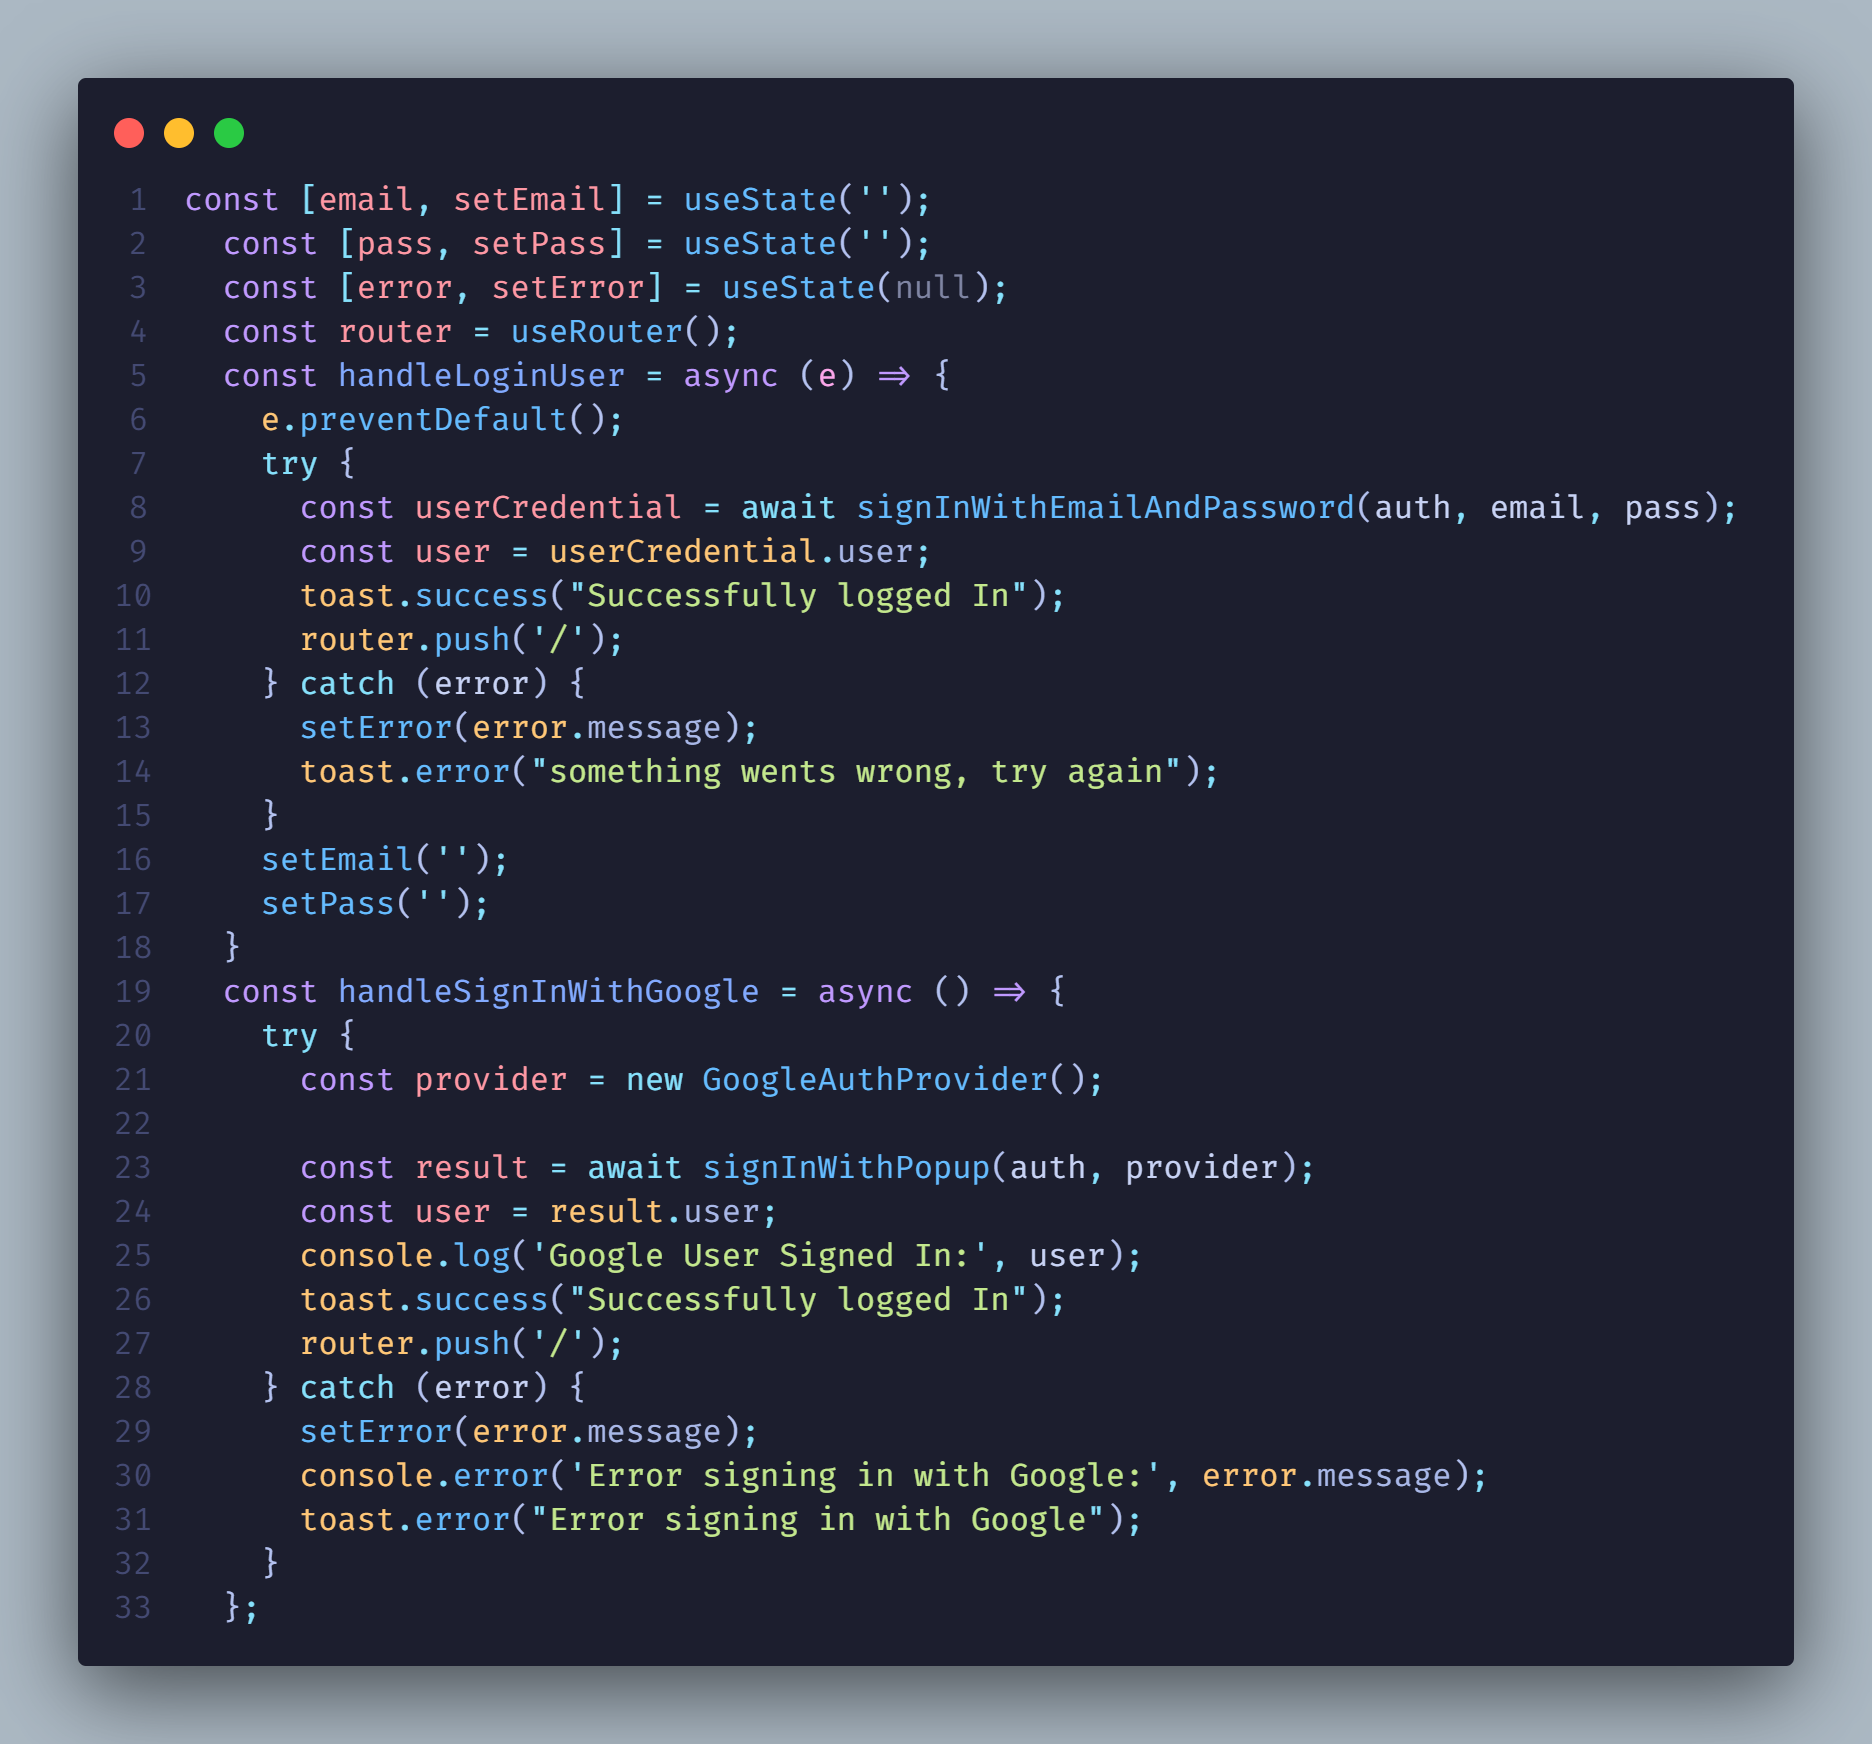
\includegraphics[width=0.9\textwidth]{./figures/implementation/login2.png}
    \caption{Login Component Code Structure}
    \label{fig:login_component}
\end{figure}

\subsection{Authentication Methods}
\begin{itemize}
    \item \textbf{Email/Password Login}:
    \begin{itemize}
        \item Uses Firebase's \texttt{signInWithEmailAndPassword}
        \item Success: Redirects to home page with success toast
        \item Error: Displays error message and toast notification
        \item Form reset after submission
    \end{itemize}
    
    \item \textbf{Google Sign-In}:
    \begin{itemize}
        \item Implements \texttt{signInWithPopup} with Google provider
        \item Success: Logs user data and redirects to home
        \item Error: Console logs error and shows toast notification
    \end{itemize}
\end{itemize}

\subsection{Error Handling}
\begin{itemize}
    \item Comprehensive try-catch blocks for both methods
    \item Error state updates for UI feedback
    \item Toast notifications for user feedback
    \item Console logging for development debugging
\end{itemize}

\subsection{Security Considerations}
\begin{itemize}
    \item Form reset after submission
    \item Protected routing after successful login
    \item No password persistence in state
    \item Secure Firebase authentication methods
\end{itemize}

\section{User Registration Implementation}

The signup component provides both email/password and Google-based registration functionality with comprehensive user profile management.

\subsection{State Management}
\begin{itemize}
    \item \texttt{useState} hooks for form control:
    \begin{itemize}
        \item \texttt{name}: Stores user's display name
        \item \texttt{email}: Stores email input
        \item \texttt{pass}: Stores password input
        \item \texttt{error}: Tracks registration errors
    \end{itemize}
    \item Router instance for navigation control
\end{itemize}

\begin{figure}[H]
    \centering
    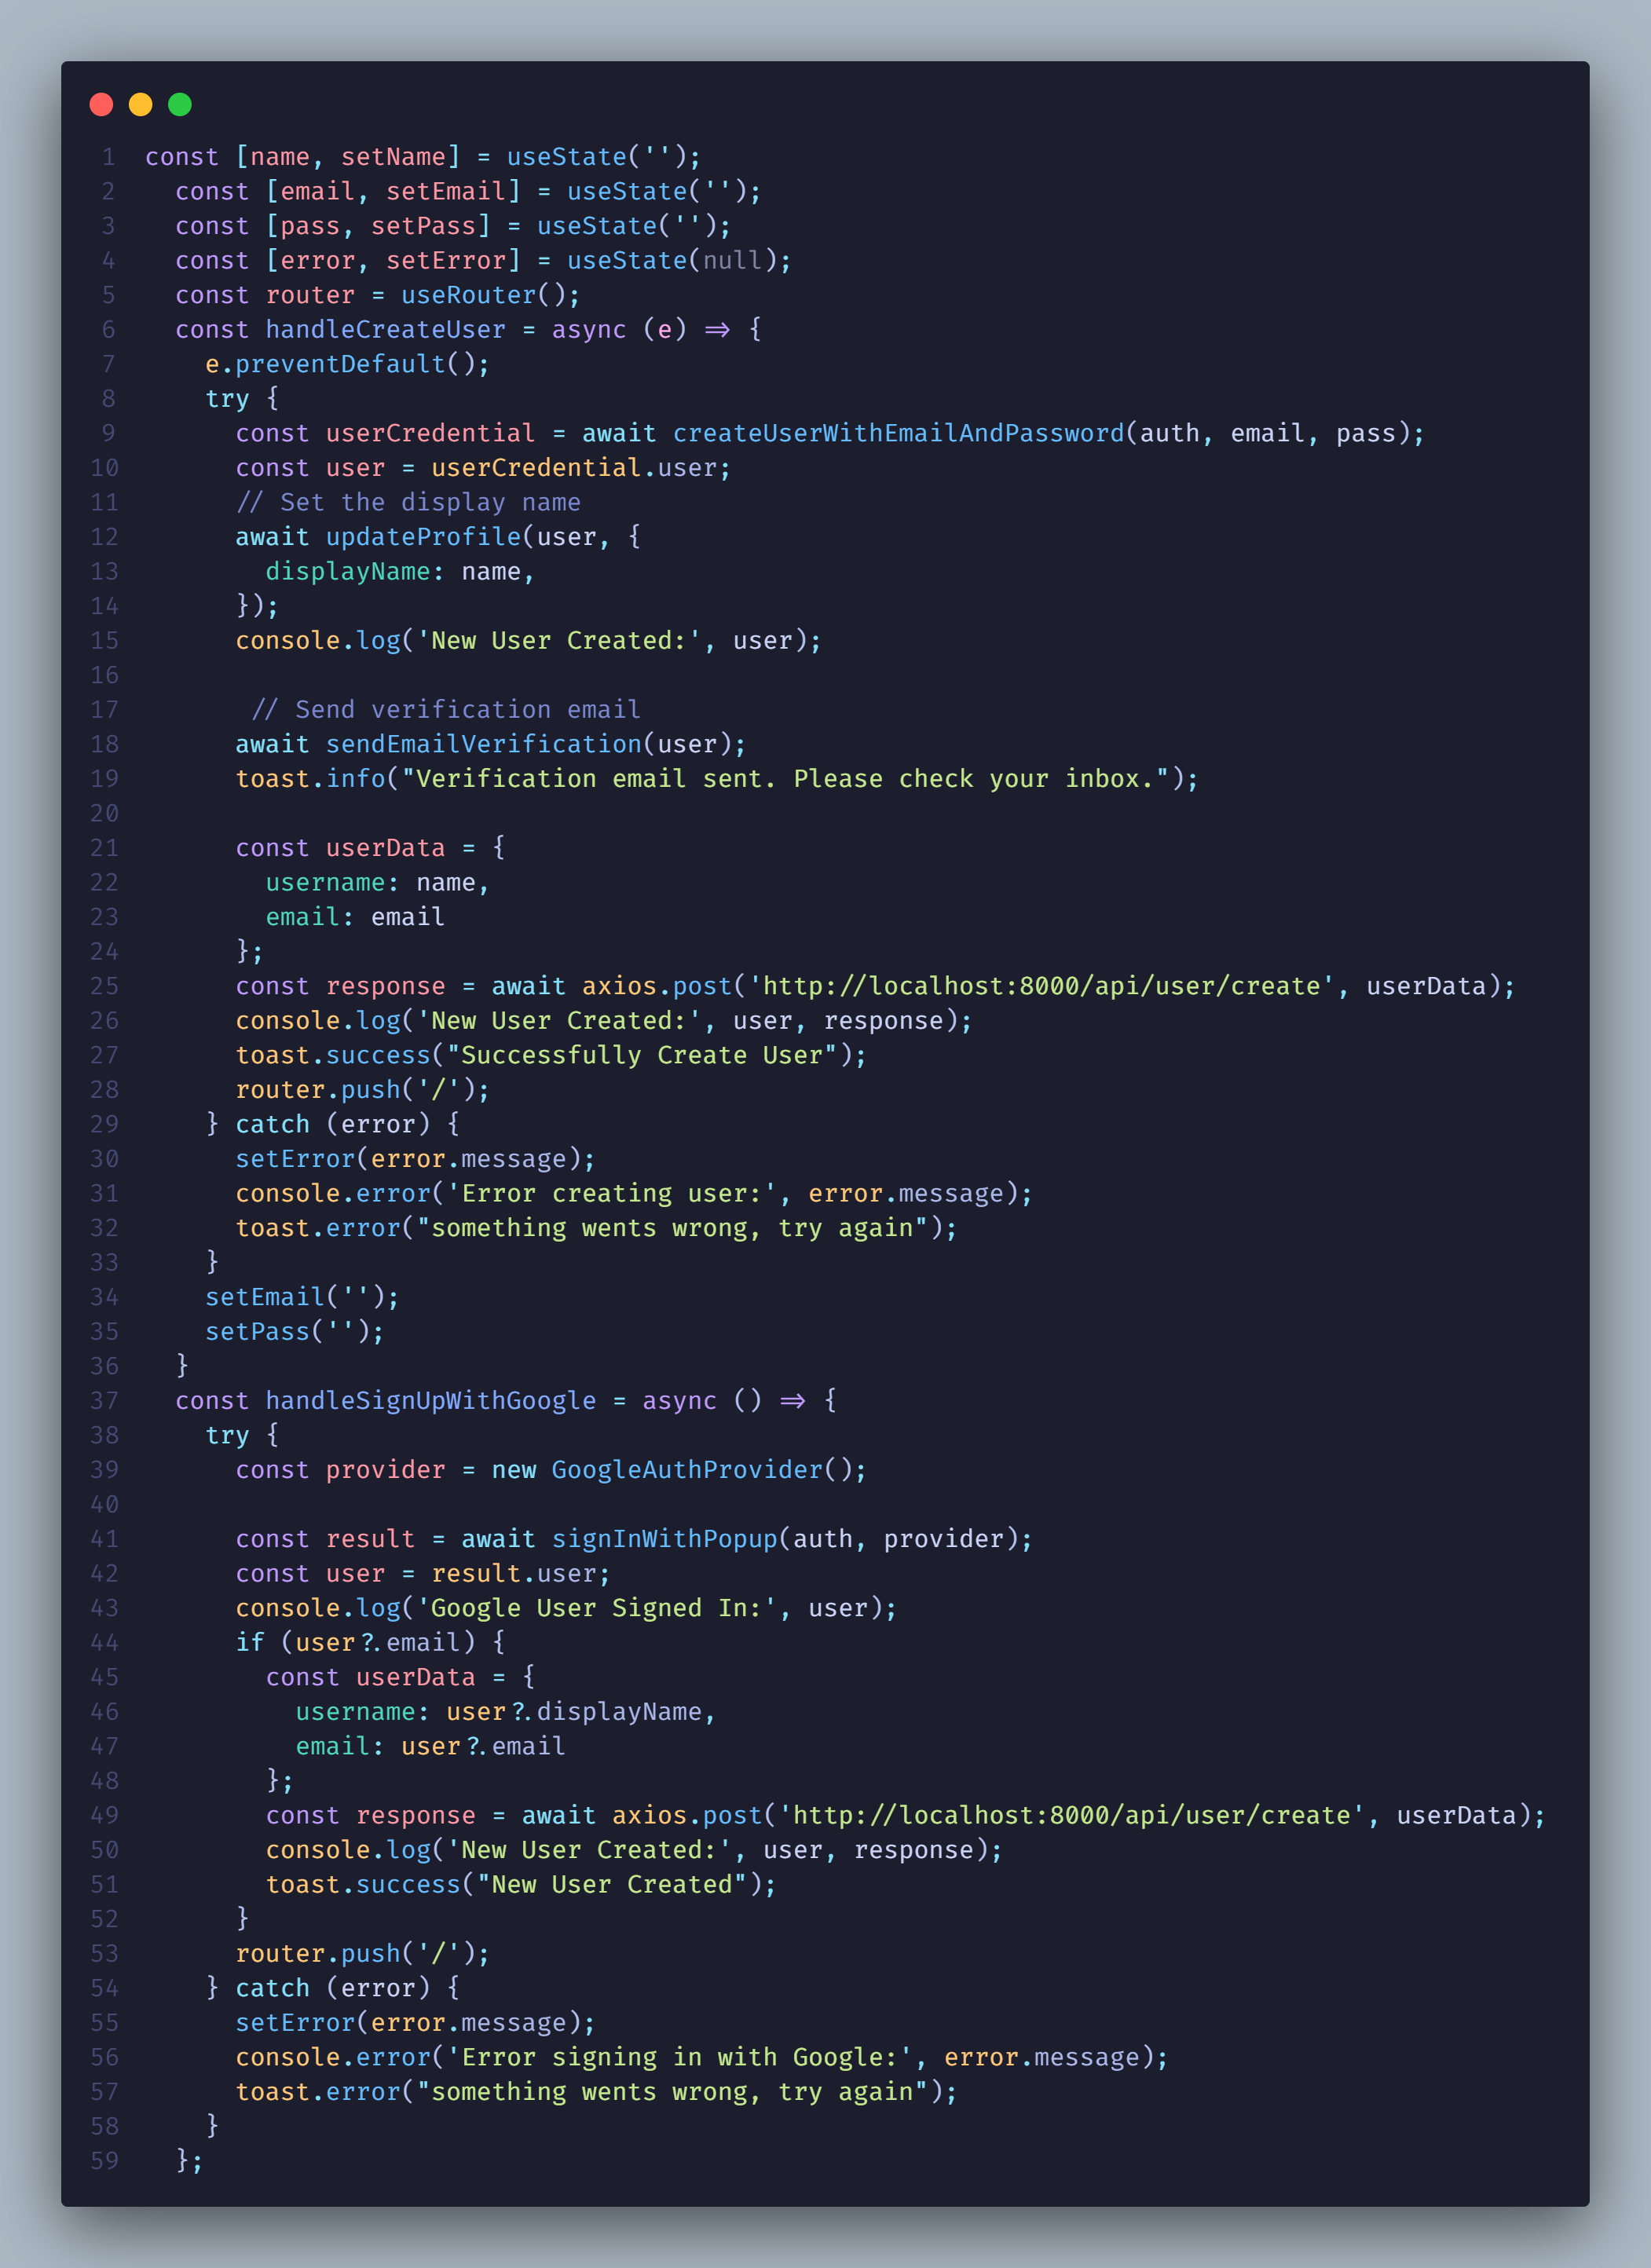
\includegraphics[width=0.9\textwidth]{./figures/implementation/signup.png}
    \caption{User Registration Code Structure}
    \label{fig:signup_component}
\end{figure}

\subsection{Registration Methods}
\begin{itemize}
    \item \textbf{Email/Password Registration}:
    \begin{itemize}
        \item Uses Firebase's \texttt{createUserWithEmailAndPassword}
        \item Sets display name via \texttt{updateProfile}
        \item Sends verification email automatically
        \item Creates backend user record via API
        \item Success: Redirects to home with success toast
    \end{itemize}
    
    \item \textbf{Google OAuth Registration}:
    \begin{itemize}
        \item Implements \texttt{signInWithPopup} with Google provider
        \item Automatically captures display name and email
        \item Creates backend user record via API
        \item Success: Redirects to home with success toast
    \end{itemize}
\end{itemize}

\subsection{Error Handling}
\begin{itemize}
    \item Comprehensive try-catch blocks for both methods
    \item Error state updates for UI feedback
    \item Toast notifications for user feedback
    \item Console logging for development debugging
    \item Form reset after email/password submission
\end{itemize}

\subsection{Security Features}
\begin{itemize}
    \item Email verification requirement
    \item Secure password handling (not persisted in state)
    \item Protected routing after successful registration
    \item Backend API integration for data consistency
\end{itemize}

\subsection{Data Flow}
\begin{itemize}
    \item Frontend to Firebase authentication
    \item Profile data to backend API (\texttt{/api/user/create})
    \item Console logging for development tracking
    \item Verification email delivery system
\end{itemize}

\section{API Routes Configuration}

The PHP code configures API routes for a travel application using Laravel, including:

\begin{itemize}
    \item User Routes: Create users, retrieve by email, assign roles
    \item Package Routes: Create, retrieve, update, delete  
    \item Hotel Routes: Create, retrieve, update, delete
    \item Flight Routes: Create, retrieve, delete
    \item Tour Guide Routes: Create, retrieve, delete
    \item Booking Routes: Create, retrieve by email
\end{itemize}

All routes use the \texttt{api} middleware group.

\begin{figure}[H]
  \centering
  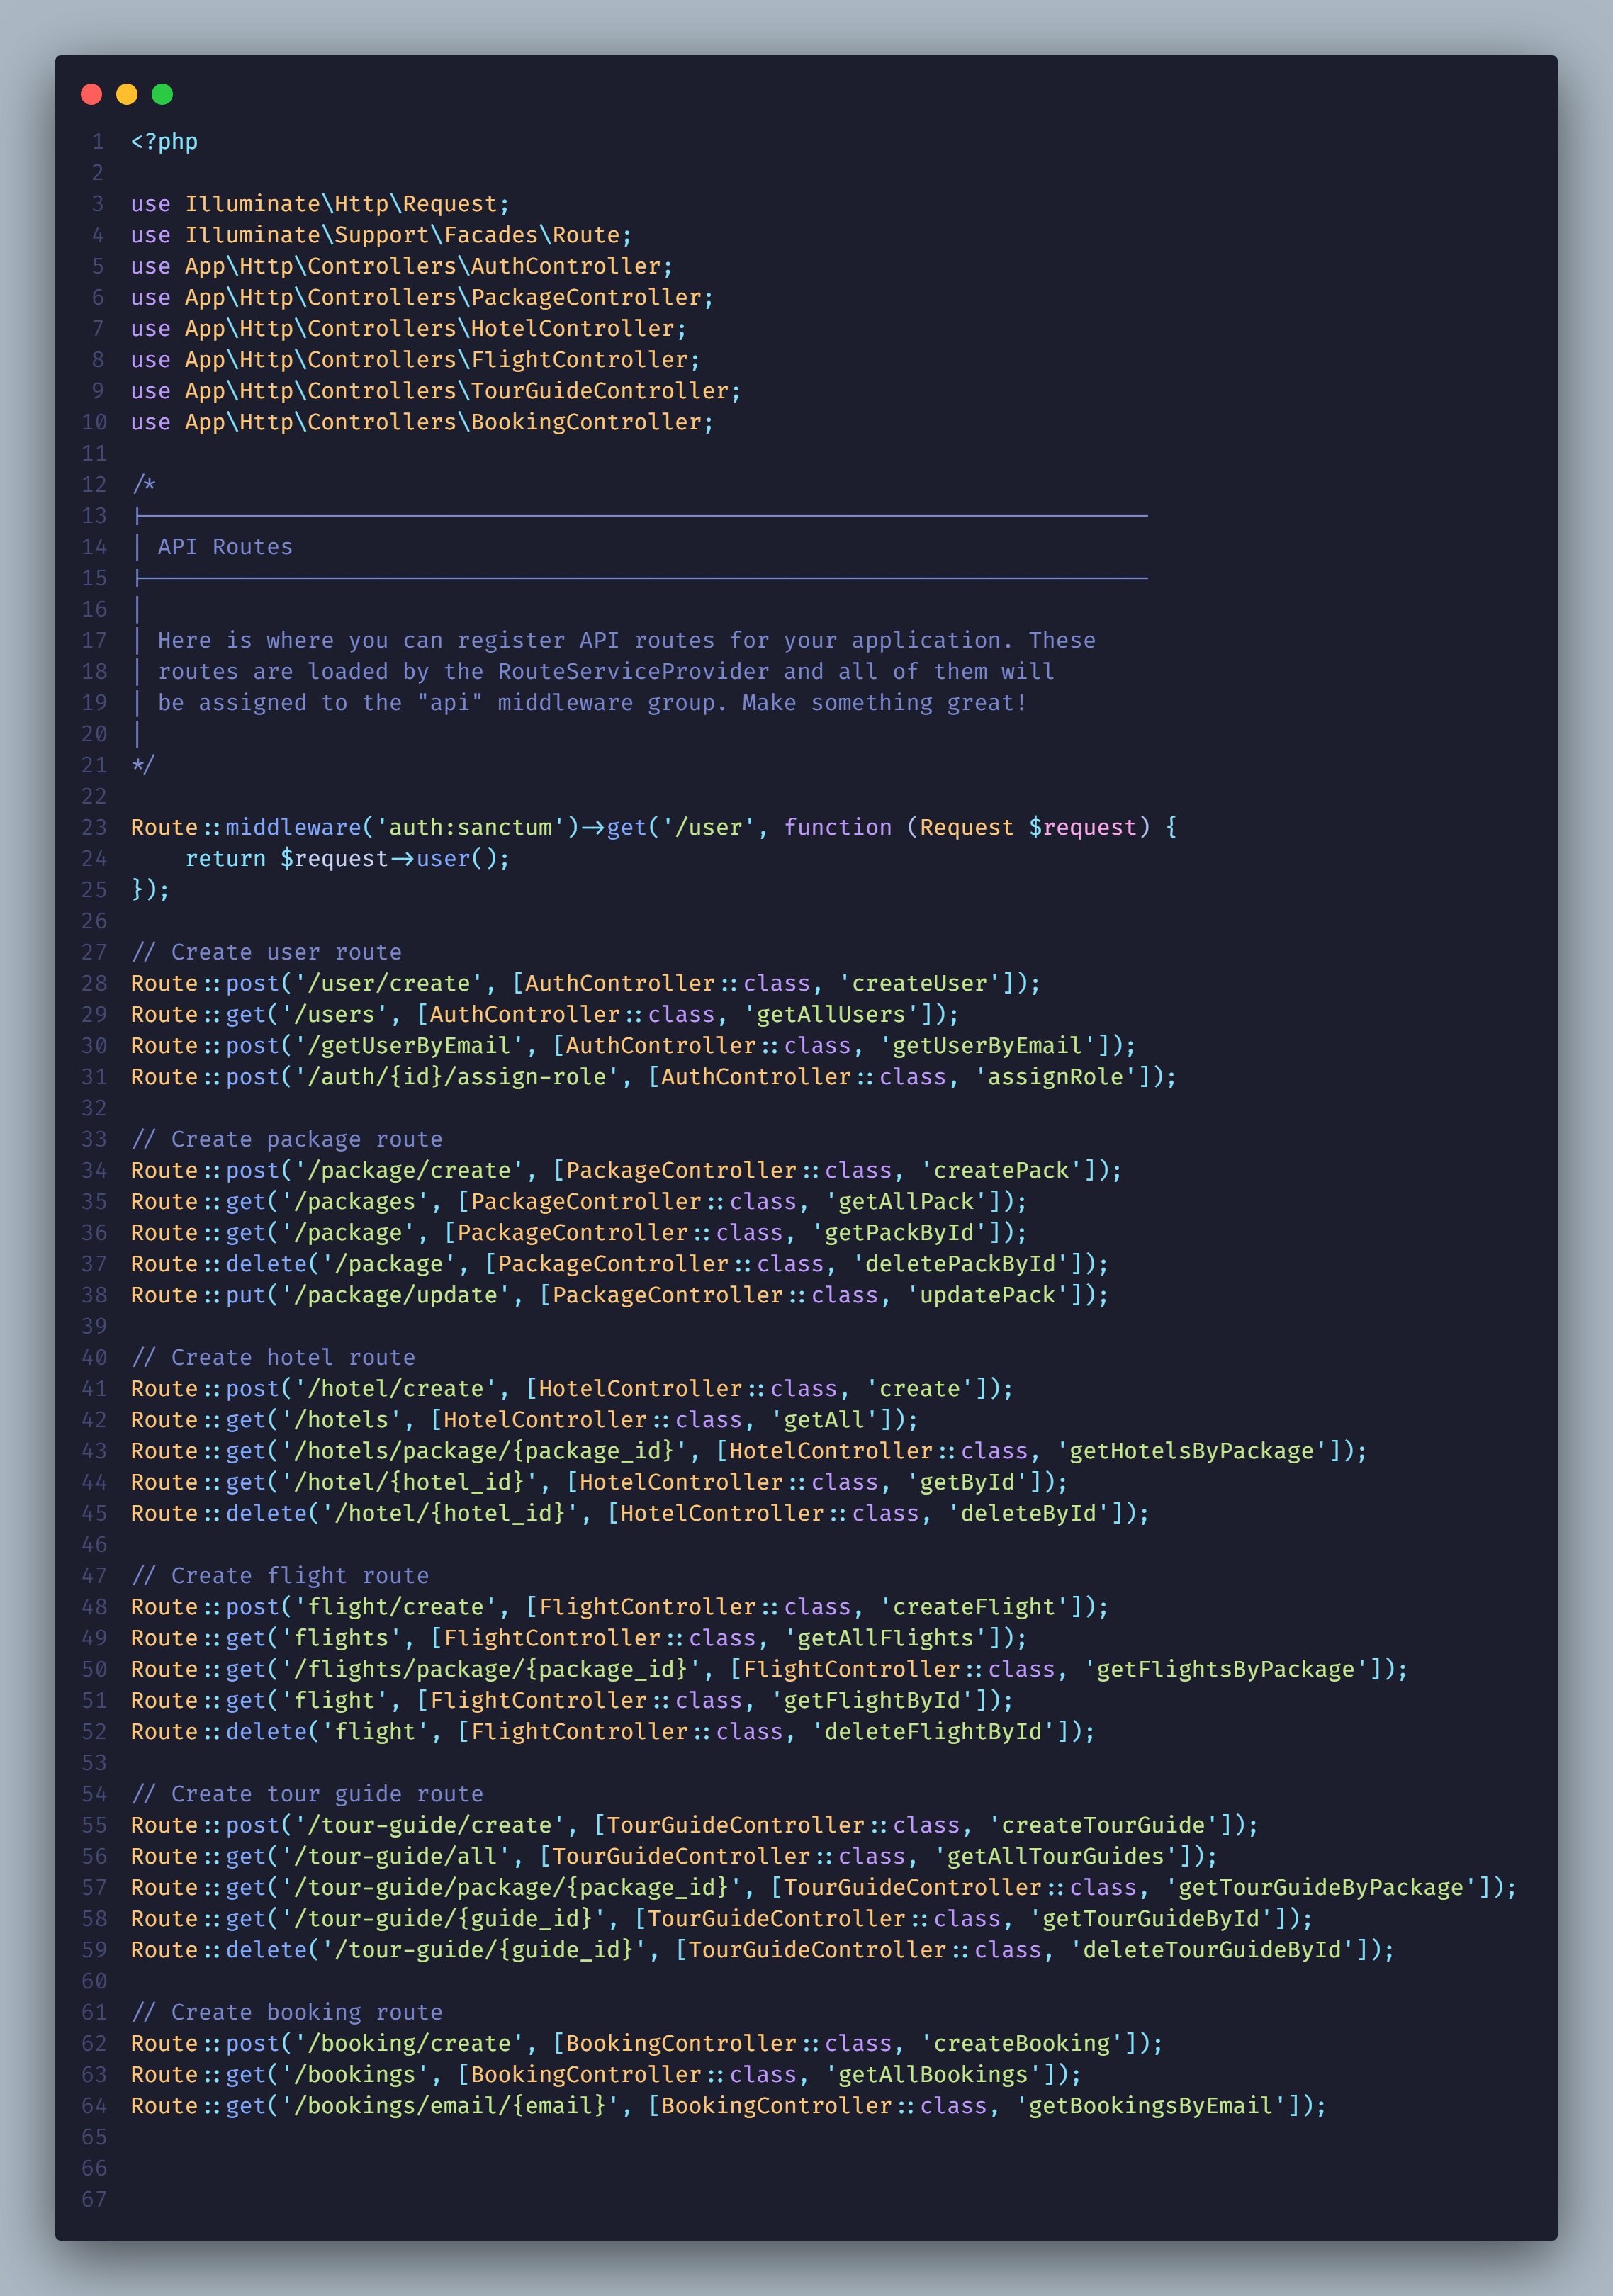
\includegraphics[width=1.0\textwidth]{./figures/implementation/api.png}
  \caption{API Routes Configuration Code Structure}
  \label{fig:api_routes}
\end{figure}

\section{Auth Controller Implementation}

The Auth Controller handles user authentication and role management operations. Key features include:

\subsection{Key Methods}
\begin{itemize}
    \item User creation with email, username, and role assignment
    \item Retrieval of all users with role information
    \item User lookup by email address
    \item Role assignment for existing users
\end{itemize}

\begin{figure}[H]
    \centering
    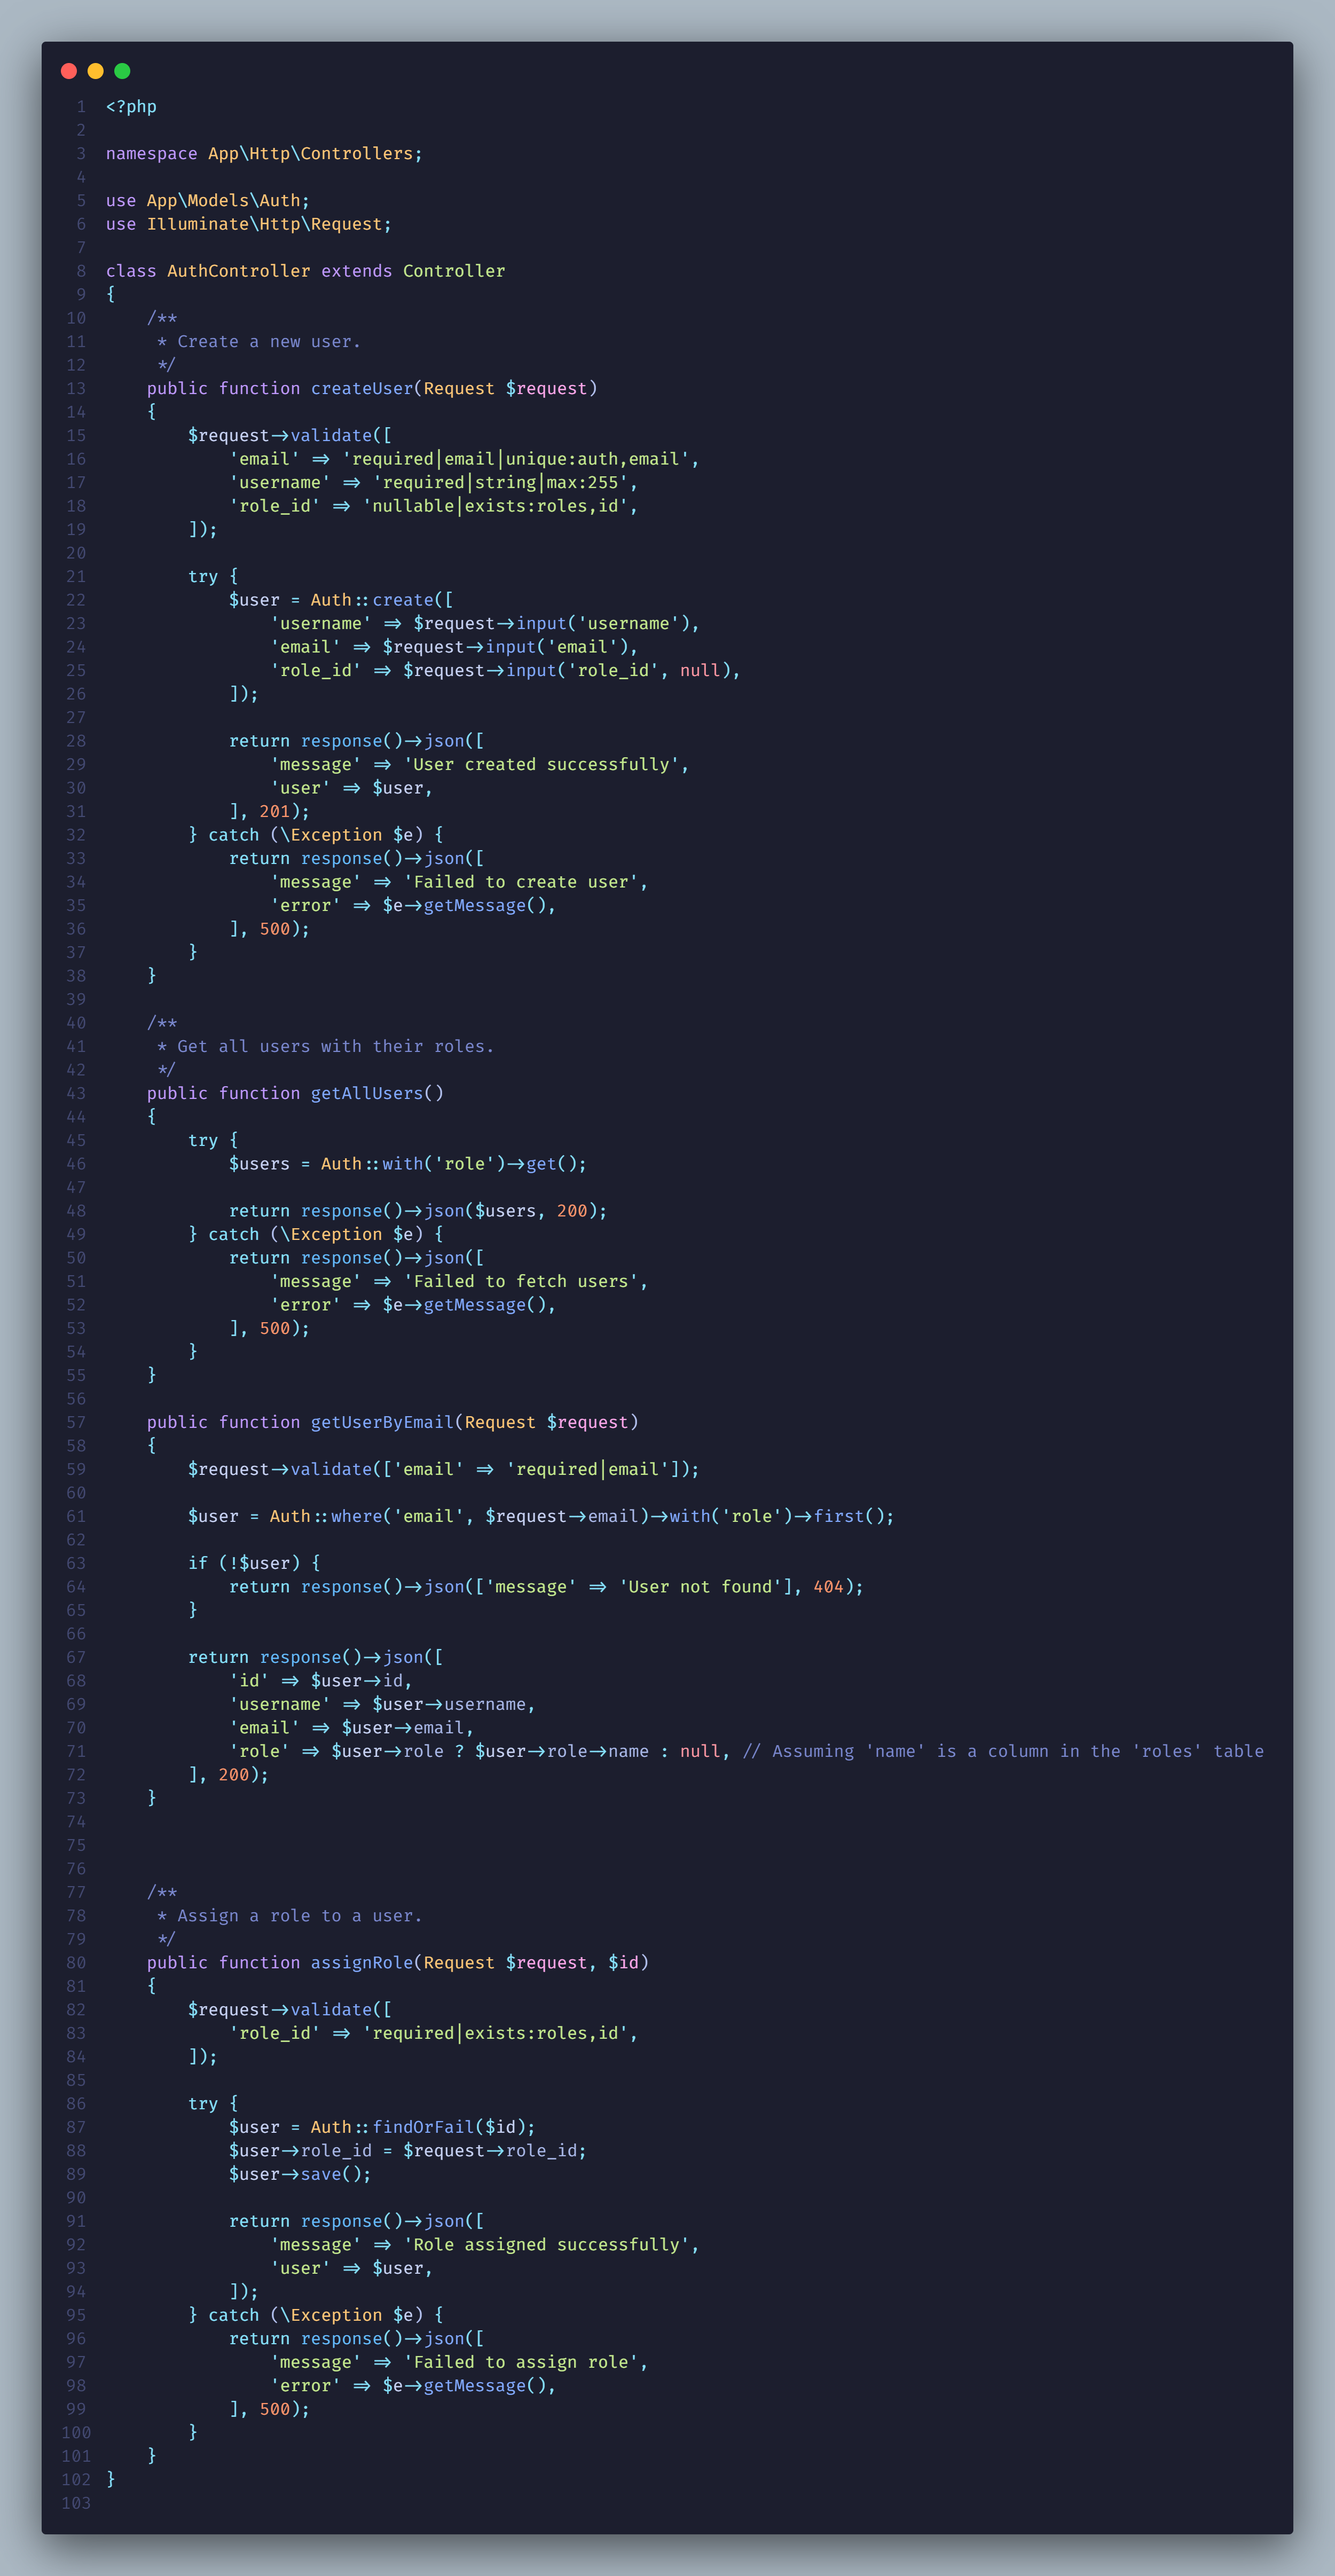
\includegraphics[width=1.0\textwidth]{./figures/implementation/Auth Controller.png}
    \caption{Auth Controller Code Structure}
    \label{fig:auth_controller}
\end{figure}

\subsection{Technical Features}
\begin{itemize}
    \item Input validation for all operations
    \item Error handling with try-catch blocks
    \item Role model integration via relationships
    \item RESTful JSON responses
\end{itemize}

\section{Package Controller Implementation}

The Package Controller manages all package-related operations in the travel application system, providing full CRUD functionality.

\subsection{Core Methods}
\begin{itemize}
    \item \texttt{createPack}: Creates new travel packages with validation
    \item \texttt{getAllPack}: Retrieves all available packages
    \item \texttt{getPackById}: Fetches specific package by ID
    \item \texttt{deletePackById}: Removes packages from the system
    \item \texttt{updatePack}: Modifies existing package details
\end{itemize}

\begin{figure}[H]
    \centering
    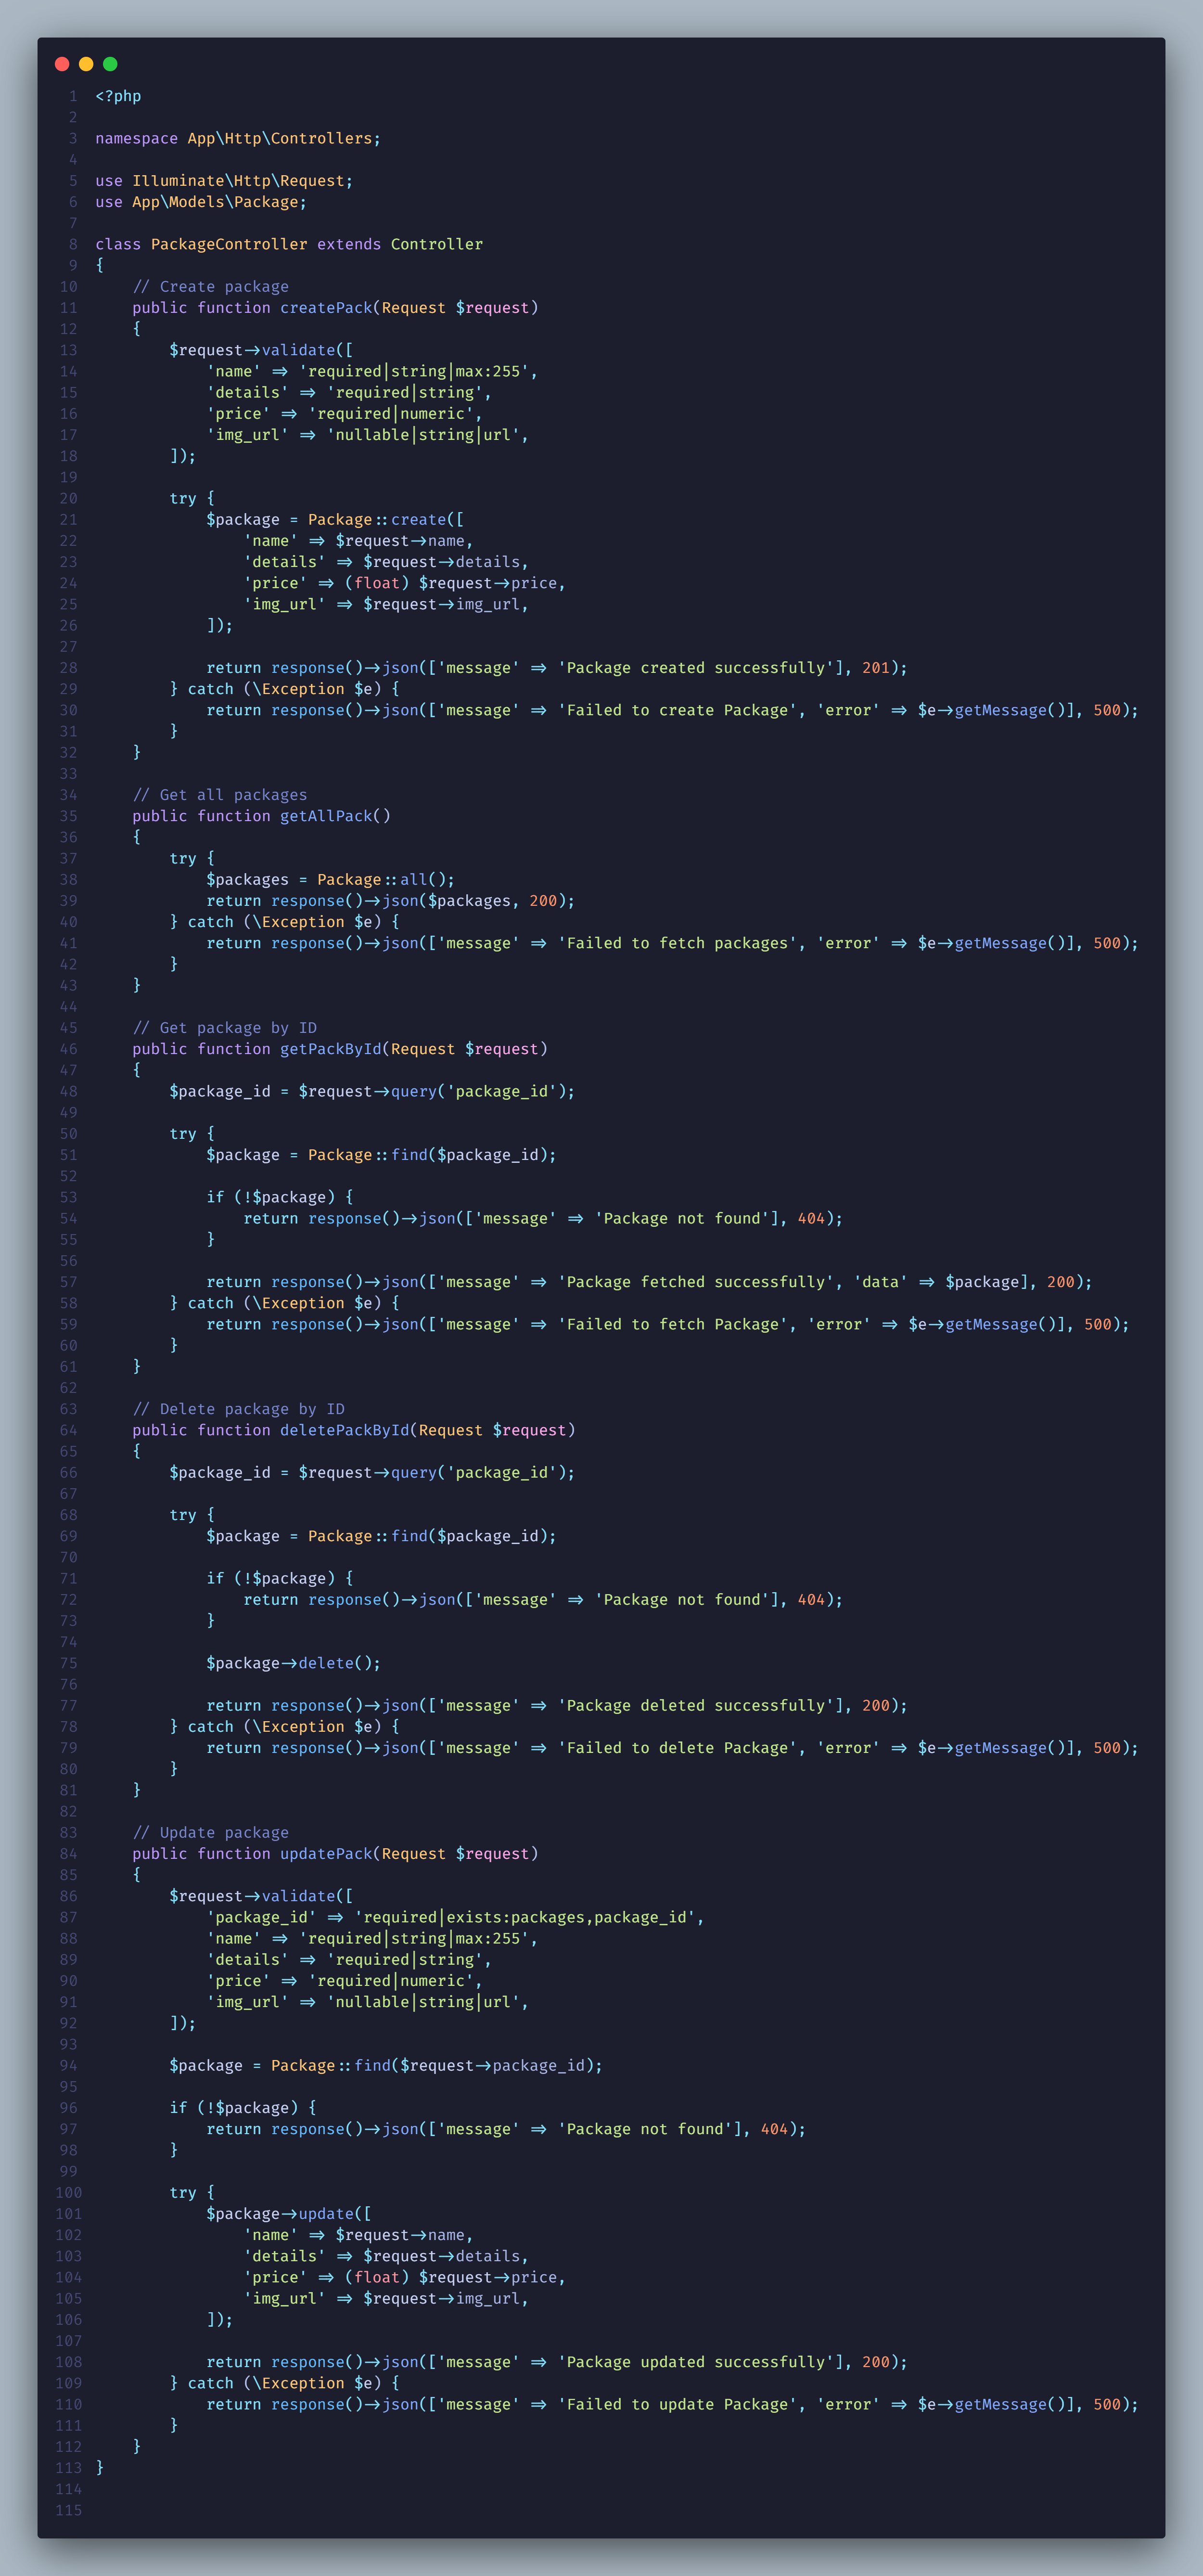
\includegraphics[width=0.9\textwidth]{./figures/implementation/Package_Controller.png}
    \caption{Package Controller Code Structure}
    \label{fig:package_controller}
\end{figure}

\subsection{Validation Rules}
\begin{itemize}
    \item Required fields:
    \begin{itemize}
        \item Package name (max 255 characters)
        \item Detailed description
        \item Price (minimum 1.0)
    \end{itemize}
    \item Optional image URL with URL validation
    \item Package ID validation for update operations
\end{itemize}

\subsection{Error Handling}
\begin{itemize}
    \item Comprehensive try-catch blocks for all operations
    \item Specific HTTP status codes:
    \begin{itemize}
        \item 200: Successful operations
        \item 400: Package not found
        \item 500: Server errors
    \end{itemize}
    \item Detailed error messages in JSON responses
\end{itemize}

\subsection{Data Processing}
\begin{itemize}
    \item Automatic price conversion to float
    \item Conditional image URL handling
    \item Proper type casting for all inputs
    \item Database transaction safety
\end{itemize}

\subsection{API Responses}
\begin{itemize}
    \item Consistent JSON response structure
    \item Success messages for all operations
    \item Error details included in failure cases
    \item Data payload for retrieval operations
\end{itemize}

\section{Booking Management System}

The booking management system handles comprehensive data processing for travel reservations. The system architecture follows a structured computer process model to ensure reliable data handling.

\subsection{Core Processes}
\begin{itemize}
    \item Data representation and information processing
    \item Comprehensive data management and tracking
    \item Flexible data modification capabilities
\end{itemize}

\begin{figure}[H]
    \centering
    
\includegraphics[width=0.9\textwidth]{./figures/implementation/booked.png}
    \caption{Booking System Code Structure}
    \label{fig:booking_system}
\end{figure}

\subsection{Key Features}
\begin{itemize}
    \item 20 modular processing components for different scenarios
    \item Uniform data handling architecture across all modules
    \item Standardized process for information representation
    \item Consistent data modification interfaces
\end{itemize}

\subsection{Technical Implementation}
The system implements:
\begin{itemize}
    \item Reusable process templates for various booking scenarios
    \item Data validation at each processing stage
    \item Audit trails for all data modifications
    \item Scalable architecture for high transaction volumes
\end{itemize}

\section{Booking Controller Implementation}

The Booking Controller manages all booking-related operations in the travel application system, providing essential CRUD functionality and query capabilities.

\subsection{Core Methods}
\begin{itemize}
    \item \texttt{createBooking}: Creates new bookings with comprehensive validation
    \item \texttt{getAllBookings}: Retrieves all booking records
    \item \texttt{getBookingsByEmail}: Finds bookings associated with a specific email
\end{itemize}

\begin{figure}[H]
    \centering
    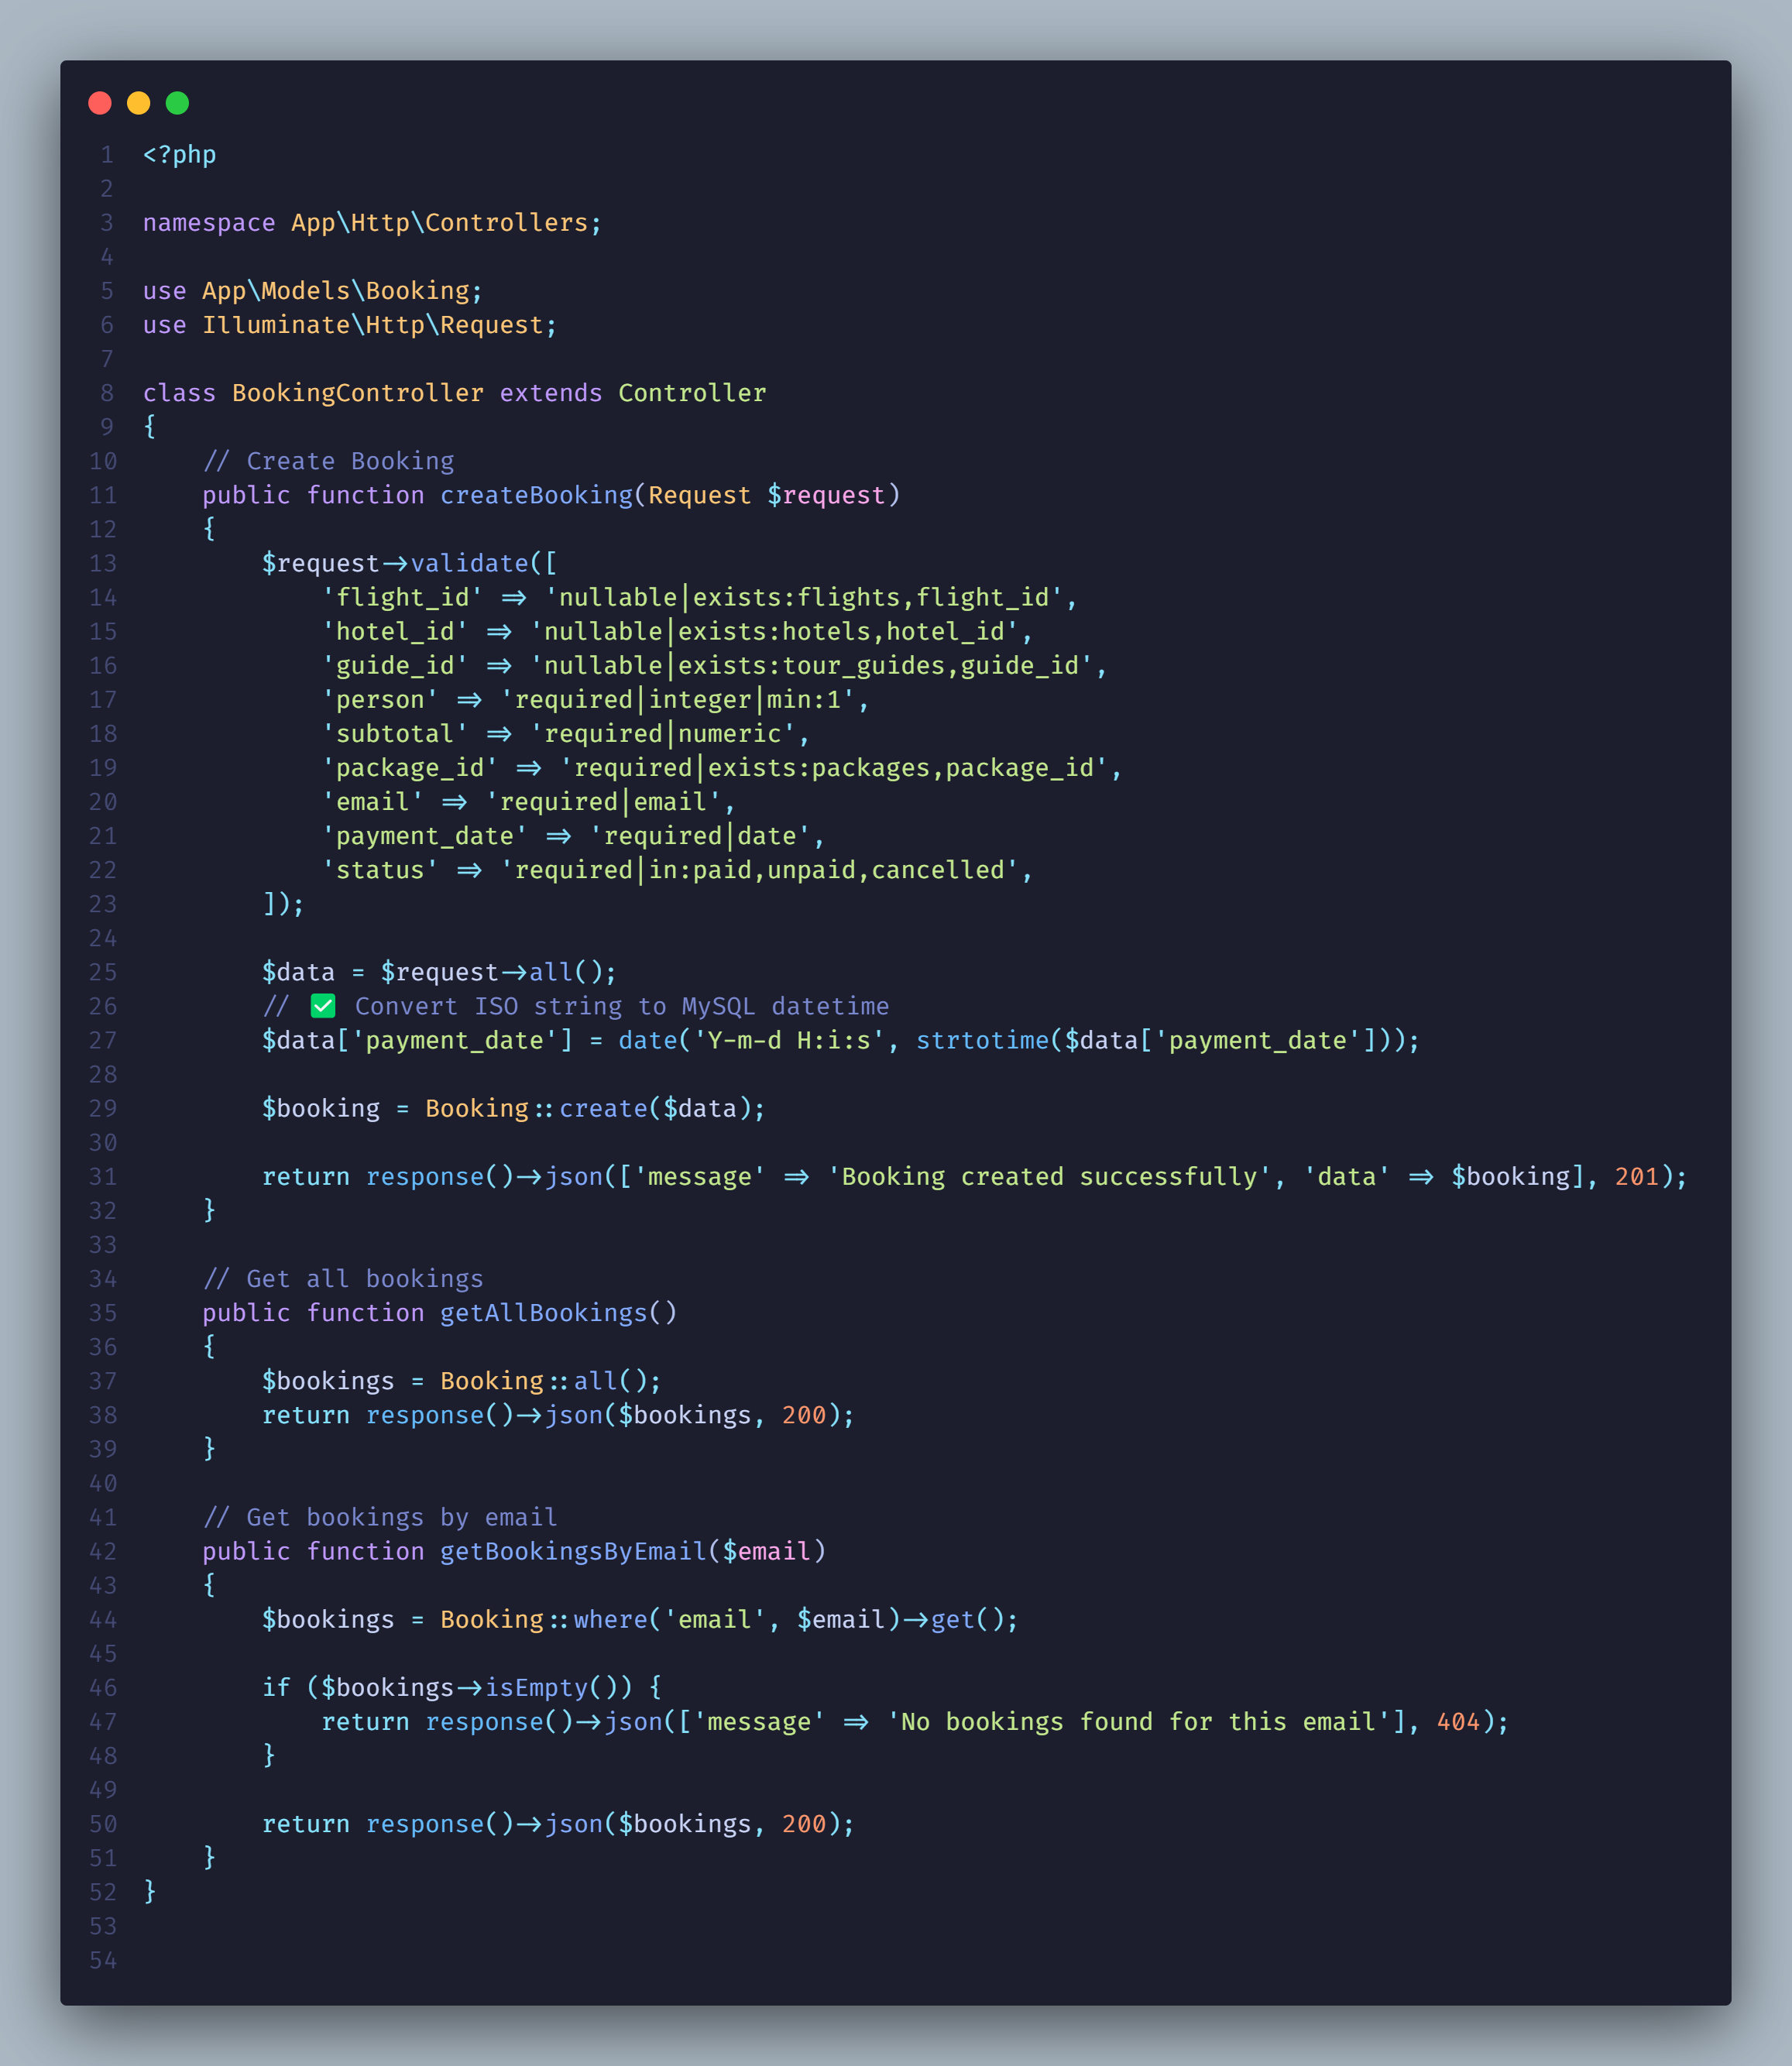
\includegraphics[width=0.9\textwidth]{./figures/implementation/Booking_Controller.png}
    \caption{Booking Controller Code Structure}
    \label{fig:booking_controller}
\end{figure}

\subsection{Technical Specifications}
\begin{itemize}
    \item \textbf{Validation Rules}:
    \begin{itemize}
        \item Foreign key checks for flights, hotels, and tour guides
        \item Required fields for person count, subtotal, and package
        \item Email format validation
        \item Payment date formatting (ISO to MySQL datetime)
        \item Status enumeration checking
    \end{itemize}
    
    \item \textbf{Data Handling}:
    \begin{itemize}
        \item Automatic date format conversion
        \item JSON response standardization
        \item Proper HTTP status codes (201, 200, 404)
    \end{itemize}
    
    \item \textbf{Error Handling}:
    \begin{itemize}
        \item Empty result detection for email queries
        \item Automatic validation error responses
    \end{itemize}
\end{itemize}

\subsection{Database Relations}
The controller interfaces with multiple database tables:
\begin{itemize}
    \item \texttt{flights} (optional relation)
    \item \texttt{hotels} (optional relation)
    \item \texttt{tour\_guides} (optional relation)
    \item \texttt{packages} (required relation)
\end{itemize}

\section{Frontend Booking Implementation}

The booking frontend interface provides users with a dynamic form to create travel reservations, integrating with multiple backend APIs.

\subsection{State Management}
\begin{itemize}
    \item \texttt{useState} hooks for all form fields:
    \begin{itemize}
        \item User email (auto-populated from authentication)
        \item Person count (default: 1)
        \item Flight, hotel, and tour guide selections
        \item Package selection from URL parameters
        \item Loading and processing states
    \end{itemize}
    \item Pagination control via \texttt{page} state
\end{itemize}

\begin{figure}[H]
    \centering
    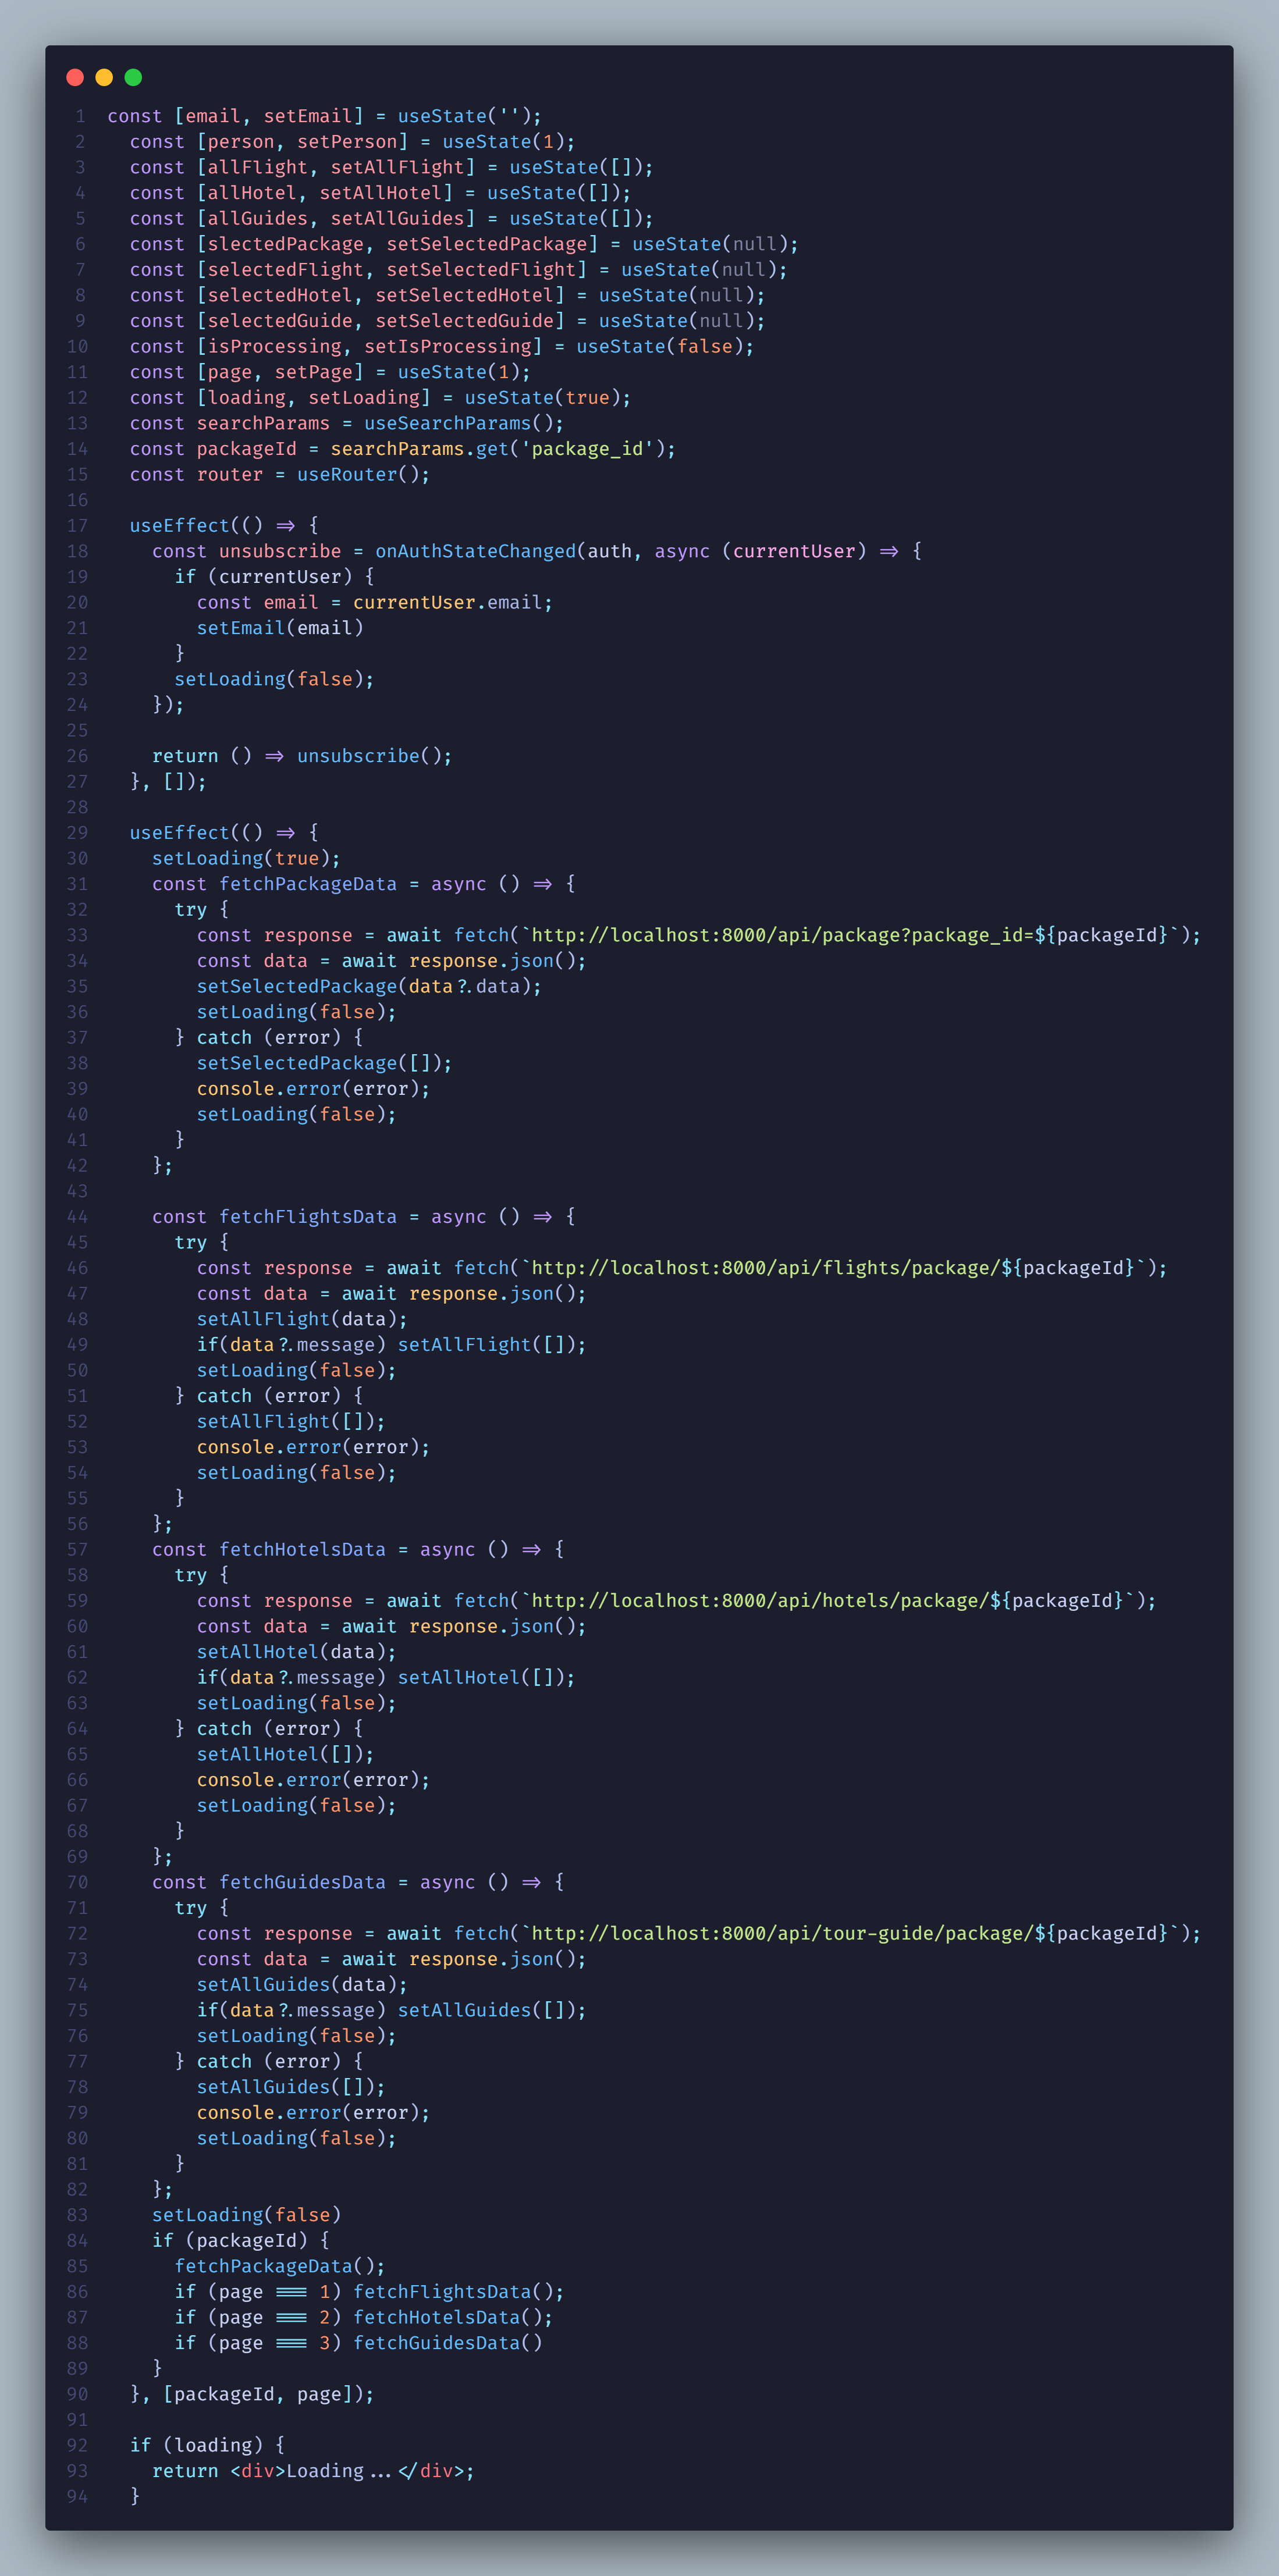
\includegraphics[width=0.9\textwidth]{./figures/implementation/booking-frontend.png}
    \caption{Booking Frontend State Management and API Integration Code Structure}
    \label{fig:booking_frontend}
\end{figure}

\subsection{API Integration}
\begin{itemize}
    \item \textbf{Data Fetching}:
    \begin{itemize}
        \item Package details from \texttt{/api/package}
        \item Available flights from \texttt{/api/flights/package}
        \item Available hotels from \texttt{/api/hotels/package}
        \item Available guides from \texttt{/api/tour-guide/package}
    \end{itemize}
    
    \item \textbf{Authentication}:
    \begin{itemize}
        \item Automatic email capture from authenticated users
        \item Loading state management during auth checks
    \end{itemize}
\end{itemize}

\subsection{Error Handling}
\begin{itemize}
    \item Empty state handling for all API responses
    \item Error logging to console
    \item Loading state management during API calls
    \item Conditional rendering based on data availability
\end{itemize}

\subsection{Component Behavior}
\begin{itemize}
    \item Dynamic data fetching based on current page
    \item Package ID extraction from URL parameters
    \item Loading indicators during data fetch operations
    \item Conditional rendering of form sections
\end{itemize}

make the content less,keep all section and images